%%%%%%%%%%%%%%%%%%%%%%%%%%%%%%%%%%%%%%%%%%%%%%%%%%%%%%%%%%%%%%%%%%%%%%%%%%%%%%%%
\chapter{ПРОЕКТИРОВАНИЕ И РЕАЛИЗАЦИЯ ПРОГРАММНОГО ОБЕСПЕЧЕНИЯ}
%%%%%%%%%%%%%%%%%%%%%%%%%%%%%%%%%%%%%%%%%%%%%%%%%%%%%%%%%%%%%%%%%%%%%%%%%%%%%%%%

%%%%%%%%%%%%%%%%%%%%%%%%%%%%%%%%%%%%%%%%%%%%%%%%%%%%%%%%%%%%%%%%%%%%%%%%%%%%%%%%
\section{Проектирование и разработка компонента регистрации новых клиентов}
%%%%%%%%%%%%%%%%%%%%%%%%%%%%%%%%%%%%%%%%%%%%%%%%%%%%%%%%%%%%%%%%%%%%%%%%%%%%%%%%

Компонент регистрации новых клиентов предназначен для решения четырех задач:

\begin{enumerate}
	\item Перенаправление всех пользователей заданной подсети на сервер регистрации.
	\item Поддержание работы сервера регистрации.
	\item Регистрация новых клиентов на удаленном сервере.
	\item Предоставление интернета зарегистрированным клиентам.
\end{enumerate}

\subsection{Проектирование архитектуры}

Для того чтобы рассматриваемый компонент был способен реализовывать поставленные задачи, было принято решение, что архитектура приложения будет разделена на три основных модуля. На рис.\ref{fig:CPArchitecture} изображена архитектура всего компонента и системы, с которыми он взаимодействует.

\begin{figure}[H]
	\centering
	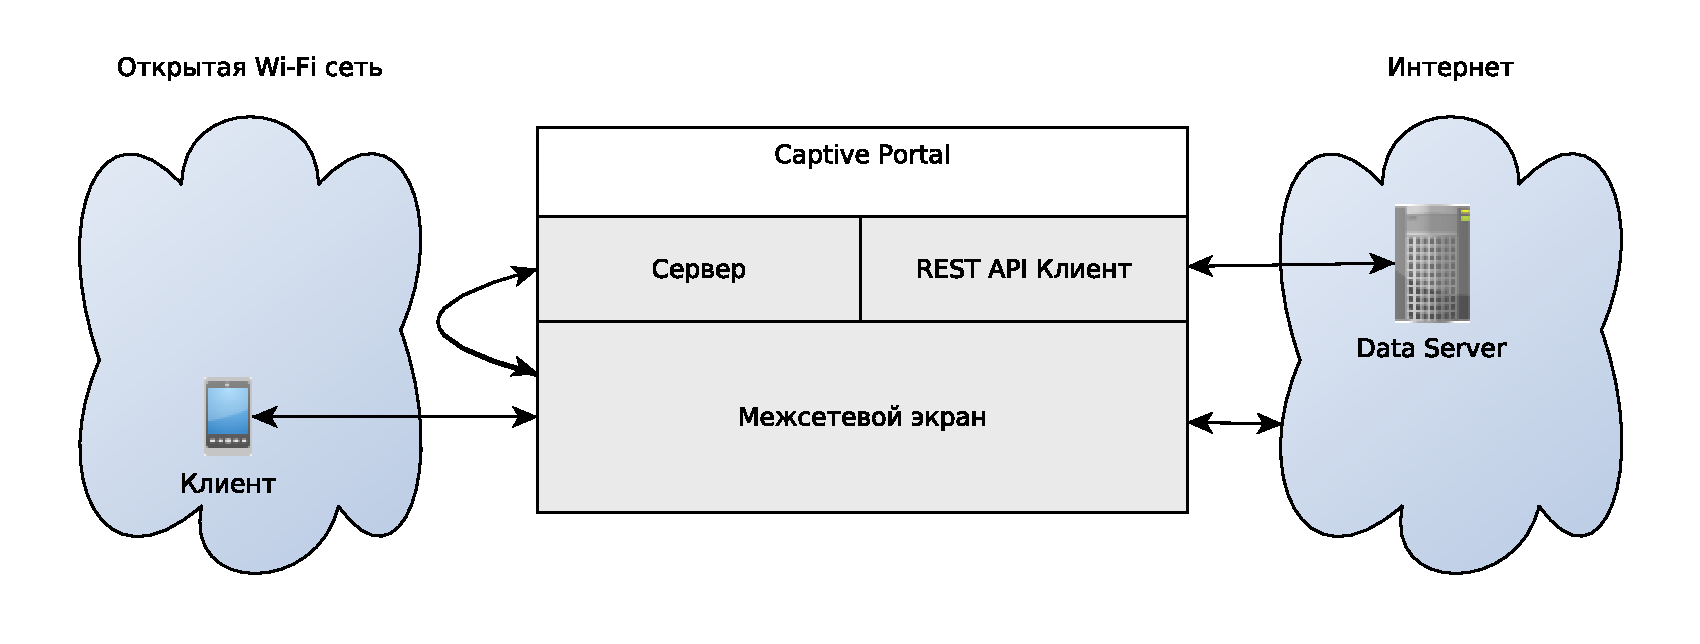
\includegraphics[width=\linewidth]{fig/CPArchitecture}
	\caption{Архитектура компонента регистрации}
	\label{fig:CPArchitecture}
\end{figure}

\textbf{Сервер} необходим для первоначального обслуживания клиентов. Данный модуль слушает 80 и 443 порты и работает по протоколу HTTP и HTTPS соответственно. В его задачи входит:

\begin{itemize}
	\item показ страницы регистрации;
	\item показ пользовательского соглашения;
	\item получение регистрационных данных;
	\item формирование события регистрации клиента;
	\item формирование события, разрешающего клиенту доступ в интернет.
\end{itemize}

\textbf{REST API Клиент} позволяет проверять MAK адрес устройства клиента в базе системы. При наличие адреса, клиенту предоставляется доступ в интернет. Данный модуль также отвечает за регистрацию новых клиентов. Передача данных между модулем и сервером системы осуществляется по протоколу HTTPS, что позволяет защитить информацию от злоумышленников.

\textbf{Межсетевой экран} осуществляет следующие функции:
\begin{itemize}
	\item перенаправляет все запросы новых клиентов на сервер Captive Portal;
	\item блокирует доступ в интернет всем не авторизованным пользователям;
	\item по команде от сервера Captive Portal предоставляет клиентам доступ в интернет.
\end{itemize}{}

\subsection{Разработка компонента}

Для организации открытой Wi-Fi сети решено использовать утилиту hostapd~\cite{hostapd}. Утилита позволяет создавать Wi-Fi точку доступа с различными параметрами путем конфигурации файла настроек. Используемый в компоненте файл настроек представлен в листинге \ref{listings:hostapd}.

Для корректной работы Wi-Fi сети необходимо наличие DHCP сервера. Роль DHCP сервера в рассматриваемом компоненте выполняет утилита dnsmasq. Для удобства обращение к серверу Captive Portal по установленному локальному имени (localcaptive) используется DNS сервер, который также реализован в утилите dnsmasq. Конфигурационный файл dnsmasq представлен в листинге \ref{listings:dnsmasq}

Предполагается, что разрабатываемый программный компонент будет устанавливаться в устройства со слабой производительностью. К таким устройствам относятся большинство домашних роутеров. Ресурсы таких устройств сильно ограничены. Они могут иметь количество памяти до 20 мб и частоту одноядерного процессора до 500 MHz. В таких условиях использование таких серверов как apache и nginx существенно замедлит работу устройства. В связи с этим, принято решение разрабатывать свой сервер на языке C++.

Для ускорения разработки и уменьшения количества ошибок было решено использовать заготовку для веб-сервера\cite{simpleServer}, написанную на языке С++ и распространяемую по лицензии MIT\cite{simpleServerMIT}. В своей работе данная заготовка использует библиотеку boost.asio\cite{boost}, которая позволяет при необходимости вносить изменения в исходный код как сервера так и библиотеки.

Технология Captive Portal подразумевает специфическую настройку межсетевого экрана в системе. В ядре Linux систем уже присутствует межсетевой экрана, который называется netfilter. Один из вариантов его настройки - использование консольной утилиты iptables. В листинге \ref{listings:iptables} приведен скрипт, который осуществляет необходимые настройка netfilter.

На рис.\ref{fig:CPUML} представлена диаграмма классов компонента регистрации

\begin{figure}[H]
	\centering
	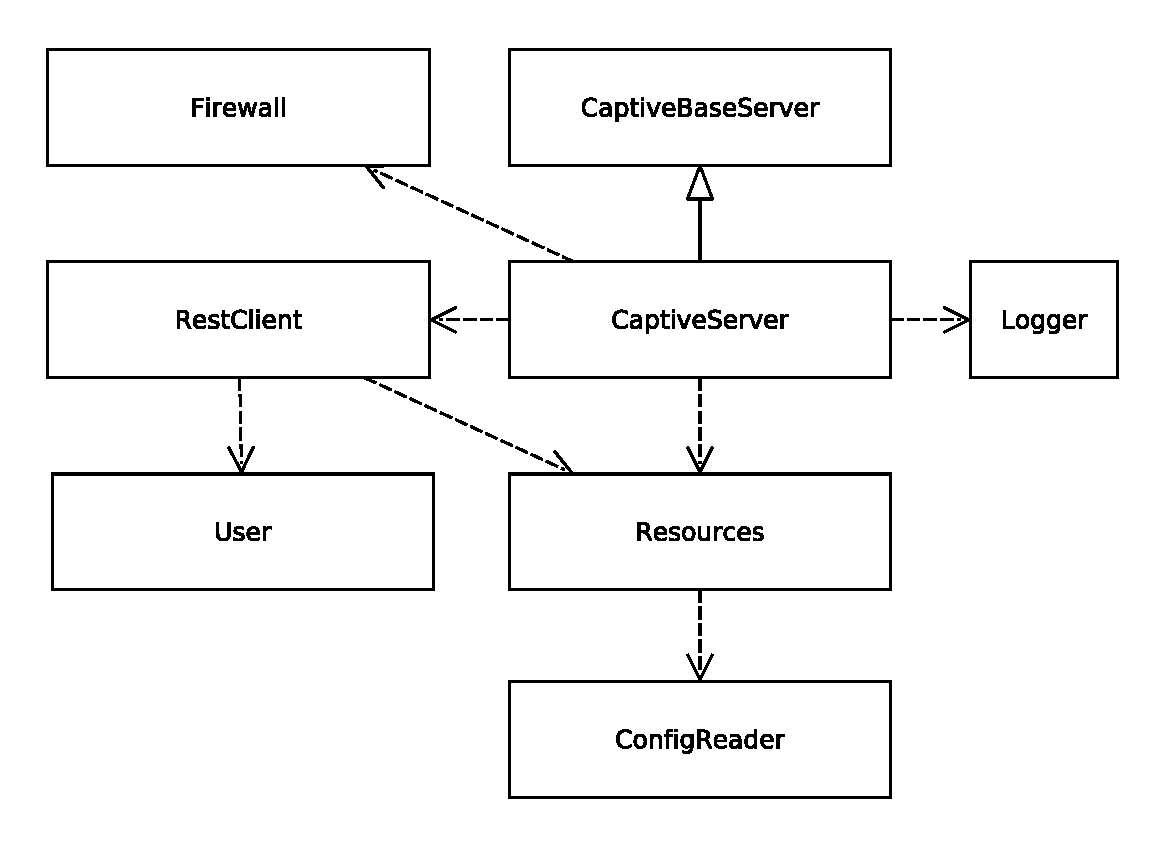
\includegraphics[width=\linewidth]{fig/CPUML}
	\caption{Диаграмма классов компонента регистрации}
	\label{fig:CPUML}
\end{figure}

Рассмотрим каждый класс и наиболее значимые методы по отдельности.

\textbf{CaptiveBaseServer.}

Базовый класс выполняет функции по инициализации полей класса и настройке сетевого фильтра. Так же в его функции входит возврат исходных настроек netfilter, после прекращения работы программы.

\textbf{CaptiveServer.}

Функцией этого класса является поддержание работоспособности сервера и выдача команд межсетевому экрану и REST API клиенту.

\textit{static void defaultGet (std::shared\_ptr <typename  SimpleWeb::Server <socket\_type>::Response> response, std::shared\_ptr <typename SimpleWeb::Server <socket\_type>::Request> request)}. Метод вызывается при получении GET запроса на сервер. Его функция - в зависимости от mac-адреса устройства вернуть страницу регистрации, или пропустить клиента в интернет. Исходный код метода представлен в листинге \ref{listings:cp}

\textit{template <class socket\_type> static void registerPost (std::shared\_ptr <typename SimpleWeb::Server <socket\_type> ::Response> response, std::shared\_ptr <typename SimpleWeb::Server <socket\_type> ::Request> request)}. Метод вызывается при получении на сервер POST запроса. Это происходит во время регистрации клиентов. Полученные данные отправляются на сервер для регистрации нового клиента. При получении положительного ответа, клиенту предоставляется доступ в интернет.

\textbf{Firewall.}

Объект этого класса выполняет функции сетевого экрана, позволяющие блокировать клиентам доступ в интернет до момента получения команды из класса CaptiveServer.

\textit{bool pass\_mac(const std::string\& ip)}. Метод позволяет открыть доступ в интернет клиенту с адресом \textit{ip}.

\textit{bool saveIptablesRules(std::string fileName)}. Входным значением является имя файла, для сохранения предыдущих настроек сетевого фильтра. Метод использует утилиту iptables-save. Возвращает true при успешном завершении операции.

\textit{bool Firewall::loadIptablesRules(std::string fileName)}. Входным значением является путь к файлу, в котором хранятся настройки сетевого фильтра. В работе используется утилита iptables-restore.

\textit{std::string exec(const char\* cmd)}. Метод исполняет команду \textit{cmd} в системе.

\textit{std::string mac\_by\_ip(const std::string\& ip)}. Позволяет получить mac-адрес клиента по заданному \textit{ip}. Для получения mac-адреса используется arp таблица, хранящаяся в системе.

\textbf{RestClient.}

Данный класс регистрирует на сервере новых клиентов и проверяет наличие MAC адреса в базе данных сервера таргетированной рекламы.

Метод \textit{bool RestClient::isClientExist(std::string mac)} получает в качестве параметра MAC адрес устройства клиента в виде AA:BB:CC:DD:EE:FF. Его задача установить зарегистрирован ли данный MAC в системе. Возвращаемое значение равно true если адрес уже существует. В противном случае возвращается false.

Метод \textit{bool RestClient::registerClient(User user)} получает в качестве параметра объект класса User и совершает попытку его регистрации на сервере. В случае успеха возвращается true, иначе false.

\textbf{User.}

Отвечает за данные, полученные от клиента при регистрации. Поля данного класса отправляются на сервер для регистрации нового клиента.

\textbf{Resources.}

Класс, реализующий паттерн проектирования Singleton. Единственный экземпляр этого класса содержит информацию о всех ресурсах, записанных в конфигурационном файле и необходимых в других компонентах системы.

\textbf{ConfigReader.}

Объект этого класса позволяет считывать конфигурационный файл, сформированный по правилу <<ресурс = значение>>.

\textit{bool isKey(const std::string\& s) const}. Метод проверяет наличие ключа \textit{s} в конфигурационном файле.

\textbf{Logger.}

Еще один класс, реализующий паттерн проектирования Singleton. Позволяет вести логирование работы системы. Логируемые сообщения имеют один из четырех уровней, определенных в перечислении LogLevel: ERROR, WARNING, INFO, DEBUG.

Метод \textit{Logger::get(LogLevel level)} возвращает единственный экземпляр класса Logger и задает уровень логирования.

Для объектов класса переопределен оператор <<<<>>, что позволяет использовать класс следующим образом:

Logger::get(LogLevel::INFO) << System started << std::endl;

Метод \textit{std::string Logger::getTimeForFileName()} позволяет получить время, используемое в имени файла логов.

Метод \textit{std::string Logger::getTimeForFileName()} возвращает время, вставляемое перед каждым сообщением при логировании. Пример файла с логами представлен в листинге \ref{listings:CPlog}

%%%%%%%%%%%%%%%%%%%%%%%%%%%%%%%%%%%%%%%%%%%%%%%%%%%%%%%%%%%%%%%%%%%%%%%%%%%%%%%%
\section{Проектирование и разработка Wi-Fi сканера}
%%%%%%%%%%%%%%%%%%%%%%%%%%%%%%%%%%%%%%%%%%%%%%%%%%%%%%%%%%%%%%%%%%%%%%%%%%%%%%%%

В список задач Wi-Fi сканера входят:

\begin{itemize}
	\item мониторинг радиоканала на частоте 2.4 ГГц;
	\item определение новых устройств в радиусе досягаемости Wi-Fi модуля;
	\item регистрация MAC-адреса устройства на сервере таргетированной рекламы.
\end{itemize}

\subsection{Проектирование архитектуры}

Архитектура Wi-Fi сканера состоит из двух модулей: сканера Wi-Fi сети и модуля регистрации посещений. На рис.\ref{fig:WiFiScanerArch} представлена архитектура Wi-Fi сканера.

\begin{figure}[H]
	\centering
	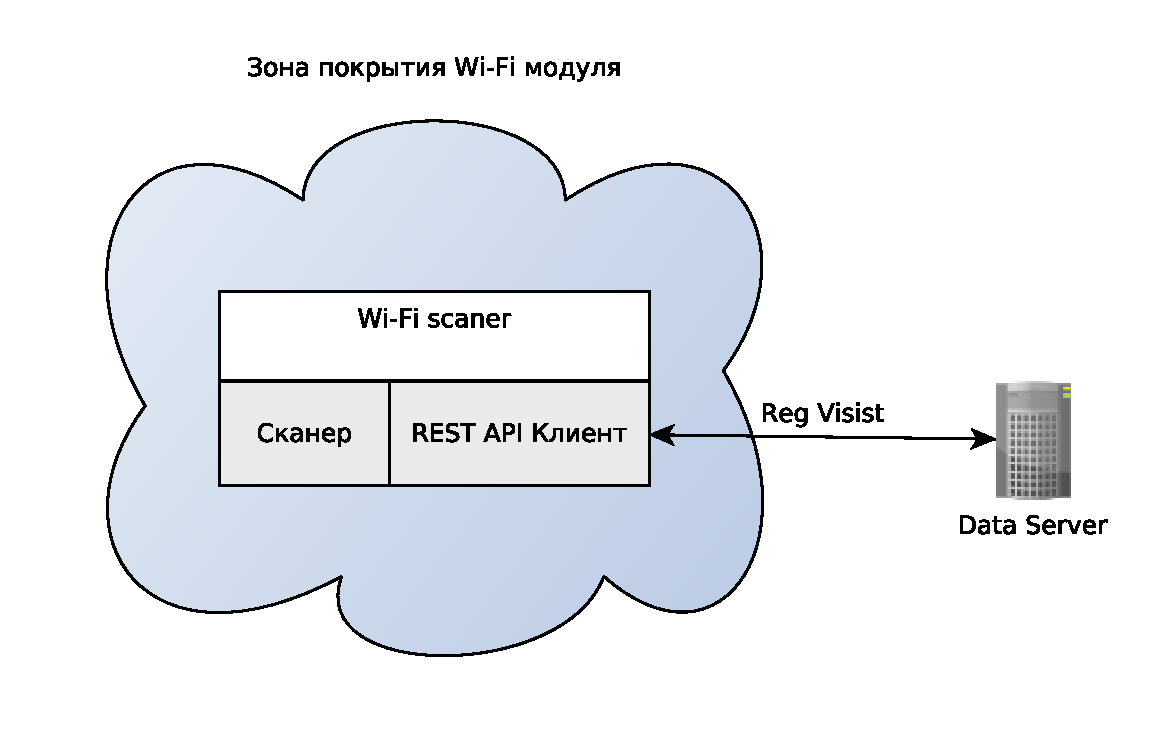
\includegraphics[width=\linewidth]{fig/WiFiScanerArch}
	\caption{Архитектура Wi-Fi сканера}
	\label{fig:WiFiScanerArch}
\end{figure}

\textbf{Сканер} осуществляет мониторинг пакетов стандарта 802.11. При выявлении пакетов от нового клиента, MAC-адрес устройства отправителя сохраняется в память для дальнейшей обработки.

\textbf{REST API клиент} регистрирует новые устройства на сервере таргетированной рекламы.

\subsection{Разработка компонента}

Wi-Fi монитор, как и компонент регистрации должен работать на устройстве со слабой производительностью. Из этого следует, что рассматриваемый компонент также следует реализовать на языке C++. Для реализации функциональности монитора решено использовать библиотеку Pcap[5]. Библиотека позволяет задавать необходимые настройка интернет адаптеру и просматривать все полученные им пакеты. Pcap используют в своей работе такие программы как Wireshark и tcpdump. Для успешного захвата всех пакетов Wi-Fi модулем, необходимо предварительно перевести его в режим монитора. Библиотека Pcap позволяет легко сделать это.

На рис.\ref{fig:WiFiScanerUML} представлена диаграмма классов Wi-Fi сканера.

\begin{figure}[H]
	\centering
	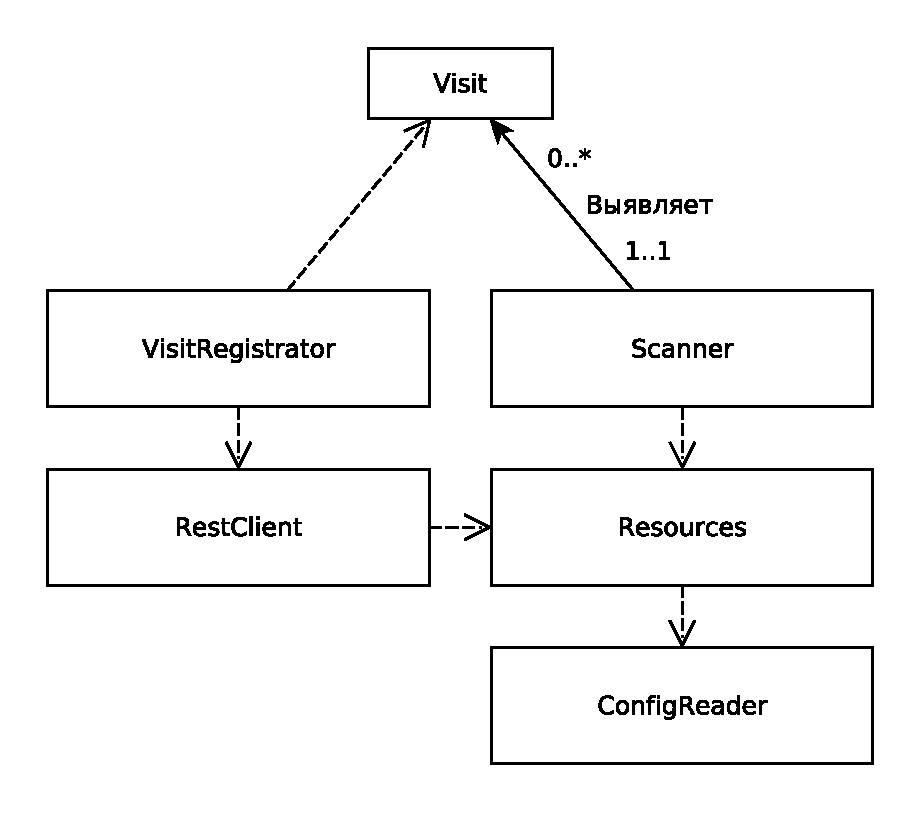
\includegraphics[width=\linewidth]{fig/WiFiScanerUML}
	\caption{Диаграмма классов Wi-Fi сканера}
	\label{fig:WiFiScanerUML}
\end{figure}

Рассмотрим каждый класс в отдельности

\textbf{Scanner}

Экземпляр данного класса устанавливает Wi-Fi модуль в режим монитора, что позволяет обрабатывать в программе все услышанные пакеты.

Метод \textit{int Scanner::start()} запускает режим мониторинга трафика и настраивает фильтрующую функцию на прием пакетов только типа Probe Request. В листинге \ref{listings:Scanner} приведен исходный код класса Scaner.

Метод \textit{void Scanner::sniffCallback(u\_char \*arg, const struct pcap\_pkthdr \*pkthdr, const u\_char \*packet)} позволяет осуществлять обработку каждого отловленного пакета. При нахождении нового устройства, во внутренней памяти создается запись типа Visit с указанием MAC-адреса устройства и временем его появления. Если запись об устройстве уже есть, то обновляется время выхода устройства из зоны действия модуля Wi-Fi.

\textbf{VisitRegistrator}

Класс осуществляет регистрацию на сервере всех устройств, которые были записаны во внутреннюю память объектом класса Scanner.

Метод \textit{void VisitRegistrator::start()} запускает работу созданного объекта. В методе осуществляется постоянная проверка списка объектов Visit с целью выявить устройство, покинувшее зону мониторинга. Это осуществляется путем проверки времени последнего обновления записи. Если запись обновлялась больше 10 минут назад, то такое посещение регистрируется на сервере и удаляется из памяти.

\textbf{Visit}

Класс является контейнером для информации о выявленном устройстве. Его полями являются: MAC-адрес устройства, время его появления, и время выхода из зоны мониторинга.

\textbf{RestClient}

Класс предназначен для регистрации посещений на удаленном сервере с помощью его REST API. 

Метод \textit{bool RestClient::sendVisit(Visit visit)} получает обьет типа Visit и с его помощью формирует POST запрос для отправки на сервер таргетированной рекламы.

Классы \textbf{Resources} и \textbf{ConfigReader} выполняют ту же функцию что и в компоненте регистрации клиентов.

%%%%%%%%%%%%%%%%%%%%%%%%%%%%%%%%%%%%%%%%%%%%%%%%%%%%%%%%%%%%%%%%%%%%%%%%%%%%%%%%
\section{Проектирование и разработка компонента генерации рекламных событий}
%%%%%%%%%%%%%%%%%%%%%%%%%%%%%%%%%%%%%%%%%%%%%%%%%%%%%%%%%%%%%%%%%%%%%%%%%%%%%%%%


\subsection{Проектирование архитектуры}

Архитектура генератора событий спроектирована исходя из выводов, сделанных при рассмотрении типовой структуры экспертных систем. В компоненте должны быть реализованы такие модули как:

\begin{itemize}
	\item модель представления знаний;
	\item средство приобретения знаний;
	\item решатель.
\end{itemize}

Решение использовать SaaS технологию для работы системы накладывает необходимость разработки веб-интерфейса. Веб-приложение, в свою очередь, является средством приобретения знаний для ЭС. В веб-интерфейсе пользователь имеет возможность сформировать правила, которые используются решателем для получения рекламных событий. Средством приобретения знаний для системы является Wi-Fi сканер.

На рис.\ref{fig:ESArch} представлена архитектура компонента генерации рекламных событий. Архитектура приложения реализована по шаблону MVC, где представлением является веб-интерфейс, моделью - база данных, а контроллером - REST API.

\begin{figure}[H]
	\centering
	\includegraphics[width=\linewidth]{fig/ESArch}
	\caption{Архитектура генератора рекламных событий}
	\label{fig:ESArch}
\end{figure}

\subsection{Разработка компонента}

Для разработки серверной части компонента решено использовать язык программирования Java и фреймворк Spring. Использование библиотеки Spring Boost значительно ускоряет этап настройки и развертывания, что делает разработку более быстрой. Одна из функций, реализованных в Spring - поддержка спецификации JPA. JPA позволяет сохранять в удобном виде java-объекты в базе данных(БД). При этом программисту не нужно задумываться о синхронизации объектов и базы данных. Это делает работу со слоем хранения программы удобной и исключает возможные ошибки при написании собственных компонентов взаимодействия с БД. В качестве реализации JPA интерфейса выбрана библиотека Hibernate. Spring фреймворк позволяет быстро настроить и использовать эту библиотеку.

Для создания веб-приложения решено использовать фреймворк Angular пятой версии. Он позволяет организовывать структуру веб приложения в компоненты, что делает ее более понятной и структурированной. Фреймворк подразумевает использование языка TypeScript, который исключает некоторые недочеты JavaScript, такие как динамическая типизация и отсутствие модульности.

\textbf{Серверная часть компонента генерации рекламных событий.}

Одним из важных компонентов серверной части является Решатель, позволяющий генерировать рекламные события. Его работа независима и заключается в периодической фильтрации клиентской базы данных с использованием имеющихся в базе знаний правил. 

Правила представлены в виде набора параметров, которыми может обладать клиент и специального типа, который позволяет фильтровать посещения клиентов. Правила бывают трех типов:

\begin{enumerate}
	\item моментальное - выполняется во время появления клиента в области действия Wi-Fi сканера
	\item по дням недели - выполняется, если клиент посещает определенный набор мест в выбранные дни недели N недель подряд.
	\item по последним дням - выполняется, если клиент посетил определенный набор мест последние N дней.
\end{enumerate}

В серверной части реализованы два модуля паттерна MVC - модель и контроллер. Модель реализована с использованием библиотеки Hibernate, что, в свою очередь, выделяет в ней два блока: блок сущностей и блок реализации JPA интерфейса. Созданные в Java коде сущности преобразуются библиотекой в базу данных. Структура базы данных представлена на рис.\ref{fig:DB}.

\begin{figure}[H]
	\centering
	\includegraphics[width=\linewidth]{fig/DB}
	\caption{Структура базы данных генератора рекламных событий}
	\label{fig:DB}
\end{figure}

Рассмотри каждую сущность более подробно.

\textit{Company} - компания потребитель, которой принадлежат определенные компоненты регистрации и Wi-Fi сканеры.  

\textit{Client} - клиент системы, зарегистрировавшийся в одной из открытых Wi-Fi сетей. Сущность хранит информацию о номере телефона, MAC-адресе устройства, возрасте  и поле клиента.

\textit{Router} - этой сущностью моет быть как Wi-Fi сканер так и компонент регистрации новых клиентов. Разграничение происходит по внутреннему полю type. Хранит информацию о своем географическом положении и компании - владельце.

\textit{Rule} - правило, сохраненное в виде набора параметров, по которому будет выявлен список целей для применения рекламного события. 

\textit{Visit} - запись о посещении клиентом определенного Wi-Fi сканера с указанием времени появления и убытия.

\textit{Action} - объект, являющийся указанием к выполнению определенного рекламного действия. В рамках выполняемой задачи этот объект является SMS сообщением. 

Контроллер позволяет совершать манипуляции с данными используя REST API интерфейс. Рассмотрим наиболее интересные контроллеры и их функции.

 \textit{ClientController} позволяет взаимодействовать с сущностью клиента. В его функции входит выполнение таких задач как создание нового клиента и проверка на наличие в базе уже существующего.

 \textit{CompanyController} взаимодействует с сущностью компании и позволяет создавать компанию и извлекать компанию по ее логину.

 \textit{VisitController} позволяет создавать посещения и просматривать имеющиеся. 

\textbf{Веб-часть компонента генерации рекламных событий.}

Для веб части реализованы два модуля. Первый модуль отвечает за авторизацию представителя компании-потребителя в системе и регистрацию новых пользователей. Второй компонент предоставляет пользователям возможность добавлять в систему новые правила.

\section{Резюме}

В результате процесса проектирования и разработки реализованы следующие компоненты: Wi-Fi сканер, компонент регистрации новых клиентов и компонент генерации рекламных событий с интерфейсом для формирования рекламных правил. Следующим и завершающим станет этап тестирования разработанных компонентов.